\section{Challenges}

\hidenum
\begin{frame}[noframenumbering]
\frametitle{Contents}
 \tableofcontents[currentsection,hideallsubsections]
\end{frame}
\shownum


\subsection{Challenges}

\begin{frame}
  \begin{block}{Challenges}
    \begin{itemize}[<+-|alert@+>]
      \item Perceptions.
      \item Library loading.
      \item Profiling.
    \end{itemize}
  \end{block}
\end{frame}


\begin{frame}
  \begin{block}{Covariance Revisited: Distributed Data Parameter Calibration}
    \begin{center}
     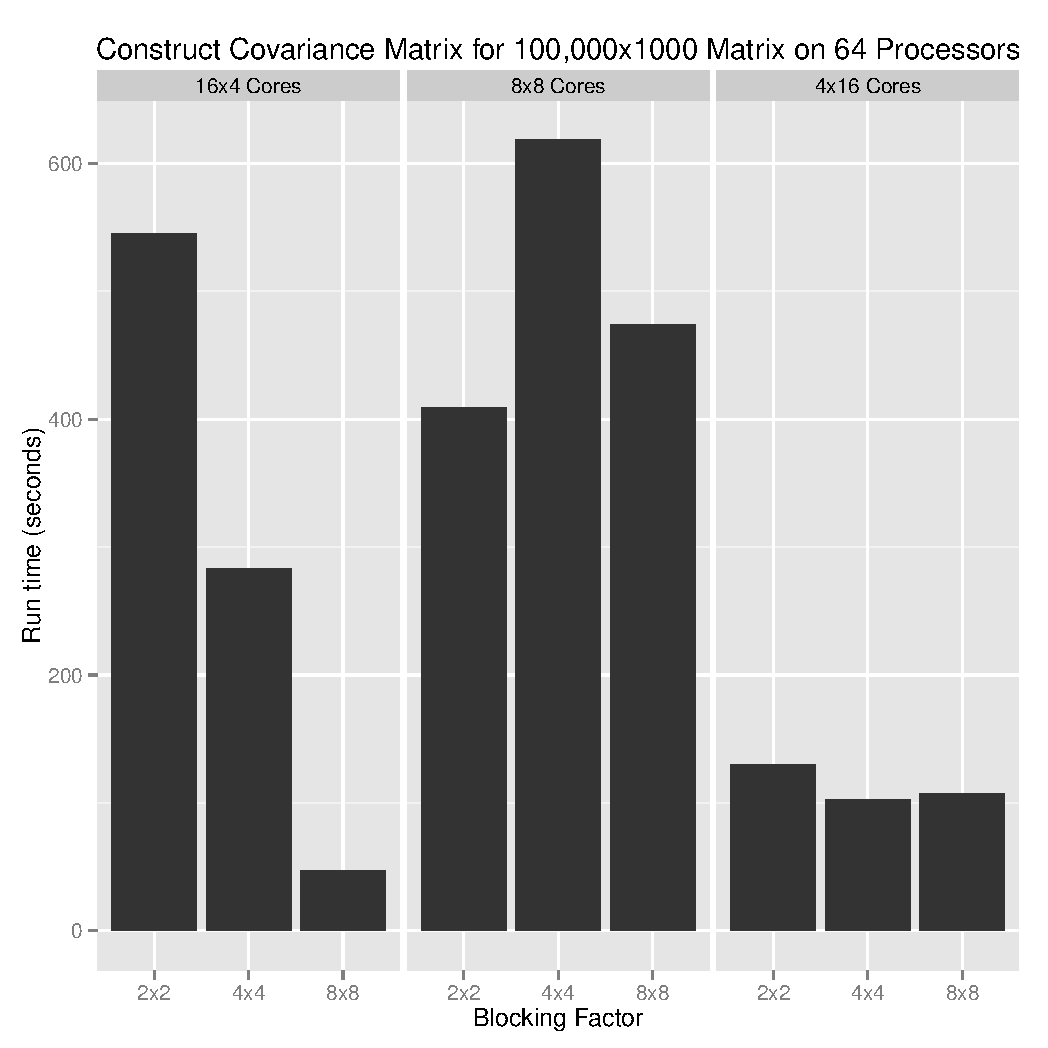
\includegraphics[width=10cm, height=7cm]{pics/cov_param}
    \end{center}
  \end{block}
\end{frame}

\begin{frame}
  \begin{block}{Tutorials}
  \begin{itemize}
    \item {\small XSEDE13, July 22, San Diego, California, USA }
    \item {\small SC13, November 17-22, Denver, Colorado, USA }
  \end{itemize}
  \end{block}
  \begin{block}{Invited Talks}
  \begin{itemize}
    \item {\small JSM 2013, August 3-8, Montr\'eal, Qu\'ebec }
    \item {\small IASC, Aug 22-23, Seoul}
    \item {\small World Statistics Congress, August 25-30, Hong Kong }
  \end{itemize}
  \end{block}
\end{frame}
  
\hidenum
\begin{frame}[noframenumbering]
 \begin{block}{Thanks for coming!}
 \begin{center}
     {\Large Questions?}\\[.6cm]
     \url{https://github.com/wrathematics/talks/blob/master/user2013/elevatingr.pdf?raw=true}
  \end{center}
 \end{block}
\end{frame}
